% !TeX program = LuaLaTeX
\documentclass[12pt,oneside]{book}
\usepackage{comment} % enables the use of multi-line comments (\ifx \fi) 
\usepackage{lipsum} %This package just generates Lorem Ipsum filler text. 
\usepackage[left=0.5in,right=1.5in]{geometry}
\usepackage{amsmath}
\usepackage{amssymb,amsthm}  % assumes amsmath package installed
\newtheorem{theorem}{Theorem}
\newtheorem{corollary}{Corollary}
\usepackage{graphicx}
\usepackage{tikz}
\usetikzlibrary{arrows}
\usepackage{verbatim}
\usepackage[numbered]{mcode}
\usepackage{float}
\usepackage{tikz}
    \usetikzlibrary{shapes,arrows}
    \usetikzlibrary{arrows,calc,positioning}

    \tikzset{
        block/.style = {draw, rectangle,
            minimum height=1cm,
            minimum width=1.5cm},
        input/.style = {coordinate,node distance=1cm},
        output/.style = {coordinate,node distance=4cm},
        arrow/.style={draw, -latex,node distance=2cm},
        pinstyle/.style = {pin edge={latex-, black,node distance=2cm}},
        sum/.style = {draw, circle, node distance=1cm},
    }
\usepackage{xcolor}
\usepackage{mdframed}
\usepackage[shortlabels]{enumitem}
\usepackage{indentfirst}
\usepackage{hyperref}
\usepackage{mhchem}
\usepackage{titlesec}
\usepackage{fontspec}
\usepackage{titlesec, blindtext, color}
\usepackage{tcolorbox}
\usepackage{caption}
\usepackage{sidenotes} 
\usepackage{esdiff}
\renewcommand{\thesubsection}{\thesection.\alph{subsection}}
\usepackage{esvect}

\newenvironment{problem}[2][Problem]
    { \begin{mdframed}[backgroundcolor=blue!8] \textbf{#1 #2} \\}
    {  \end{mdframed}}

% Define solution environment
\newenvironment{solution}
    {\textit{Solution:}}
    {}

\renewcommand{\qed}{\quad\qedsymbol}
\setlength\parindent{0pt}


\newcommand{\hsp}{\hspace{20pt}}
\titleformat{\chapter}[hang]{\Huge\bfseries}{\thechapter\hsp\textcolor[HTML]{0e4eb3}{\Huge|}\hsp}{0pt}{\Huge\bfseries}

\titleformat{\section}[hang]{\huge\bfseries}{\thesection\hsp\textcolor[HTML]{db3949}{\huge|}\hsp}{0pt}{\huge\bfseries}

%%%%%%%%%%%%%%%%%%%%%%%%%%%%%%%%%%%%%%%%%%%%%%%%%%%%%%%%%%%%%%%%%%%%%%%%%%%%%%%%%%%%%%%%%%%%%%%%%%%%%%%%%%%%%%%%%%%%%%%%%%%%%%%%%%%%%%%%
\begin{document}
\begin{titlepage}
    \newgeometry{left=7.5cm,top=1.2cm,right=1cm}
    \begin{tikzpicture}[remember picture, overlay]
    \node[opacity=1,inner sep=0pt] at (current page.center)
    {
\includegraphics[width=\paperwidth,height=\paperheight]{graphics/cover.jpg}};
    \end{tikzpicture}
    \vphantom{A}
    \vfill
    \noindent{\fontsize{35}{35} \selectfont \bfseries\sffamily\noindent\textcolor{white}{Solutions for Notes on complex function theory, Donald Sarason}}
    \\{\fontsize{20}{48} \selectfont \bfseries\sffamily \textcolor{white}{Aakash Ghosh}}
    \par
    \noindent
    \makebox[0pt][l]{\rule{1.3\textwidth}{1pt}}
    \par
    \noindent
    {\large\sffamily\textcolor{white}{Written in Pain}}
\end{titlepage}
\clearpage

%\setmainfont{KITTY CAT}
\setmainfont{Meows}

\tableofcontents

\chapter{Complex Numbers}
\section{1.1-1.2}

\begin{tcolorbox}[colback=blue!15]
    
\end{tcolorbox}

\section{1.3-1.4}
\begin{tcolorbox}[colback=blue!15]
    \textbf{Problem 1}\\

\end{tcolorbox}


\section{1.5}
\begin{tcolorbox}[colback=blue!15]
    \textbf{Problem 1}\\
    
\end{tcolorbox}





\chapter{Complex Differentiation}
\section{Notes}
\begin{enumerate}
    \item If $f$ is $\mathbb C$ differentiable, it is called holomorphic. We define:
    $$f'(z_0)=\lim_{z\to z_0}\frac{f(z)-f(z_0)}{z-z_0}$$
    \item If $f$ is holomorphic then there exists $R(z)$ such that:
        $$f(z)=f(z_0)+c(z-z_0)+R(z)\qquad \lim_{z\to z_0}\frac{R(z_0)}{|z-z_0|}=0$$
        \textbf{It is easier to work with $R(z)$ if we need to prove results related to partial derivatives}
        \begin{marginfigure}%
            \includegraphics[width=2.3\marginparwidth]{graphics/ (6).png}
        \end{marginfigure}%
    \item A holomorphic function satisfies the Cauchy Riemann($CR$) equations:
    $$\diffp{u}{x}=\diffp{v}{y}\qquad \diffp{v}{x}=-\diffp{u}{y}$$
    \item If $f$ satisfies $CR$ equations and continuity of first partial derivatives it is holomorphic. It follows that linear combinations, products, quotients and compositions of holomorphic functions are holomorphic. 
    \begin{marginfigure}%
        \includegraphics[width=2.3\marginparwidth]{graphics/ (7).png}
    \end{marginfigure}%
    \item  Let $f$ be a holomorphic function defined in the open subset $G$ of $\mathbf{C}$, and let $z_0$ be a point of $G$ such that $f^{\prime}\left(z_0\right) \neq 0$. Let $\gamma_1$ and $\gamma_2$ be curves such that $\gamma_1\left(t_1\right)=\gamma_2\left(t_2\right)=z_0$, and such that $\gamma_j$ is regular at $t_j, j=1,2$. Then the angle between $f \circ \gamma_1$ and $f \circ \gamma_2$ equals the angle between $\gamma_1$ and $\gamma_2$. If a function $f$ preserves angles between all curves, it is holomorphic and $f'\ne0$.
    \item $f$ is harmonic if
        $$\diffp[2]{f}{x}+\diffp[2]{f}{y}=0$$
        Holomorphic functions are harmonic.
    \item $v$ is harmonic conjugate of $u$ iff $u+iv$ is holomorphic.
    \begin{marginfigure}%
        \includegraphics[width=2.3\marginparwidth]{graphics/ (8).png}
    \end{marginfigure}%
\end{enumerate}
\section{2.1-2.3}

\begin{tcolorbox}[colback=blue!15]
    
\end{tcolorbox}


\section{2.4-2.6}

\begin{tcolorbox}[colback=blue!15]
    \textbf{Problem 1}\\
    At which points are the following functions differentiable:
    \begin{enumerate}
        \item $f(z)=x=Re(z)$
        \item $f(z)=\overline z$
        \item $f(z)=\overline z^2$
    \end{enumerate}
\end{tcolorbox}

\begin{marginfigure}%
    \includegraphics[width=2.4\marginparwidth]{graphics/ (1).png}
\end{marginfigure}%

It is easy to check that for each of the above function 
$\frac{\partial}{\partial x}f(z),\frac{\partial}{\partial y}f(z)$ exists and is continuous. Therefore, we just need to look for points where $CR$ equations hold,i.e. $\frac{\partial}{\partial\overline z}f=0$.
\begin{enumerate}
    \item Write $Re(z)=\frac{z+\overline z}{2}$. Differentiable at $z=0$
    \item Differentiable nowhere
    \item Differentiable at $z=0$
\end{enumerate}

\begin{tcolorbox}[colback=blue!15]
    \textbf{Problem 2}\\
    Prove $\sqrt{|xy|}$ is not differentiable at the origin even if it satisfies the $CR$ equations.
\end{tcolorbox}
\begin{marginfigure}%
    \includegraphics[width=2.4\marginparwidth]{graphics/ (2).png}
\end{marginfigure}%
In the first quadrant we have $\frac{\partial}{\partial x}f=\frac{1}{2}\sqrt{\frac{y}{x}}$. In fourth quadrant we have  $\frac{\partial}{\partial x}f=-\frac{1}{2}\sqrt{\frac{y}{x}}$. As partial derivative w.r.t $x$ is not $C^1$ at $z=0$, it is not differentiable at origin.


\begin{tcolorbox}[colback=blue!15]
    \textbf{Problem 3}\\
    Prove that the $CR$ equations in polar co-ordinates are:
    $$r\diffp{u}{r}=\diffp{v}{\theta}\quad \diffp{u}{\theta}=-r\diffp{v}{r}$$
\end{tcolorbox}
\begin{marginfigure}%
    \includegraphics[width=2.4\marginparwidth]{graphics/ (3).png}
\end{marginfigure}%
For a function $f$ we have: $x=r\cos\theta$ and $y=r\sin\theta$. Therefore:
    $$\diffp{x}{r}=\cos\theta=\frac{x}{r}\quad\diffp{y}{r}=\sin\theta=\frac{y}{r}$$
It follows that:
    $$r\diffp{f}{r}=r\left(\diffp{f}{x}\diffp{x}{r}+\diffp{f}{y}\diffp{y}{r}\right)=\left(x\diffp{f}{x}+y\diffp{f}{y}\right)$$ 
Similarly, 
$$\diffp{x}{\theta}=-r\sin\theta=-y\quad\diffp{y}{r}=r\cos\theta=x$$
and 
$$\diffp{f}{\theta}=\left(\diffp{f}{x}\diffp{x}{\theta}+\diffp{f}{y}\diffp{y}{\theta}\right)=\left(-y\diffp{f}{x}+x\diffp{f}{y}\right)$$
We get the polar forms of $CR$ equations as:
\begin{align*}
    r\diffp{u}{r}=\left(x\diffp{u}{x}+y\diffp{u}{y}\right)=\left(x\diffp{v}{y}-y\diffp{v}{x}\right)=\diffp{v}{\theta}\\
    -r\diffp{v}{r}=\left(-x\diffp{v}{x}-y\diffp{v}{y}\right)=\left(x\diffp{u}{y}-y\diffp{u}{x}\right)=\diffp{u}{\theta}
\end{align*}
\section{2.7-2.8}
\begin{tcolorbox}[colback=blue!15]
    \textbf{Problem 1}\\
    Let $f$ be holomorphic in an open disc $D$. Prove that each of those conditions force $f$ to be a constant.
    \begin{enumerate}
        \item $f'=0$ on $D$
        \item $f$ is real valued on $D$
        \item $|f|$ is constant on $D$
        \item $arg(f)$ is constant on $D$
    \end{enumerate}
\end{tcolorbox}
\begin{marginfigure}%
    \includegraphics[width=2.4\marginparwidth]{graphics/ (4).png}
\end{marginfigure}%

\begin{enumerate}
    \item Assume that $f$ is not constant. Then there exists $z_1,z_2$ such that $f(z_1)\ne f(z_2)$. Therefore, $u(z_1)\ne u(z_2)$ or $v(z_1)\ne v(z_2)$. WLOG, assume  $u(z_1)\ne u(z_2)$. Consider the function $h(\lambda)=u(\lambda z_1+(1-\lambda)z_2)$. As $h(0)\ne h(1)$, by $LMVT$, we have $\lambda\in [0,1]$ such that $h'(\lambda)\ne0\Rightarrow u'(\lambda z_1+(1-\lambda)z_2)\ne0\Rightarrow f'(\lambda z_1+(1-\lambda)z_2)\ne0$ which is a contradiction.
    \item If $f$ is real valued then $v$ is $0$. It follows that $\diffp{v}{x}=\diffp{v}{y}=0$. By $CR$ equations we have $\diffp{u}{x}=\diffp{v}{y}=0$ and $\diffp{u}{y}=-\diffp{v}{x}=0$. Therefore, $f'=0$ and by (i), $f$ is constant. 
    \item Since $|f|=r$ is constant we can write $f(x+iy)=r\cos\theta(x+iy)+ir\sin\theta(x+iy)$. We use $CR$ equations to get:
    \begin{align}
        -r\diffp{\theta}{x}\sin\theta(x,y)=r\diffp{\theta}{y}\cos\theta(x,y)\\
        -r\diffp{\theta}{y}\sin\theta(x,y)=-r\diffp{\theta}{x}\cos\theta(x,y)
    \end{align}
    Divide and rearrange to get:
    $$\left(\diffp{\theta}{x}\right)^2=-\left(\diffp{\theta}{y}\right)^2$$
    Which implies that both sides of the above equation is 0. Therefore, $\theta$ is a constant which implies $f$ is a constant. 
    \item As $arg(f)$ is constant, there exists $\lambda$ such that $u=v\lambda$. If $\lambda =0$ then $f$ is imaginary values, or $if$ is real valued, and is therefore constant. So we can assume $\lambda\ne0$. We then have:
    $$\diffp{u}{x}=\lambda\diffp{v}{x}=-\lambda\diffp{u}{y}=-\diffp{v}{y}=-\diffp{u}{x}$$
    Similarly, we get $\diffp{v}{y}-\diffp{v}{y}$. As each partial derivative is 0, by (i), $f$ is constant. 
\end{enumerate}


\begin{tcolorbox}[colback=blue!15]
    \textbf{Problem 2}\\
    Let the function $f$ be holomorphic on open set $G$. Show $g(z)=\overline{f(\overline{z})}$ is holomorphic on $\{\overline{z}|z\in G\}$ 
\end{tcolorbox}
\begin{marginfigure}%
    \includegraphics[width=2.3\marginparwidth]{graphics/ (5).png}
\end{marginfigure}%
Note that:
$$g(x,y)=\overline{f(x,-y)}=\overline{(u(x,-y),v(x,-y))}=u(x,-y),-v(x,-y)$$
It is easy to check that $\diffp{g}{x},\diffp{g}{y}$ are continuous and that $CR$ equations are satisfied 
\section{2.9-2.15}
\begin{tcolorbox}[colback=blue!15]
    \textbf{Problem 1}\\
    For what values of real $a,b,c,d$ is $u(x,y)=ax^3+bx^2y+cxy^2+dy^3$ harmonic? Determine harmonic conjugate when $u$ is harmonic.
\end{tcolorbox}
\begin{marginfigure}%
    \includegraphics[width=2.3\marginparwidth]{graphics/ (9).png}
\end{marginfigure}%
It follows from the definition that
\begin{align*}
    &\diffp[2]{u}{x}+\diffp[2]{u}{y}=0\\
    \Rightarrow&(6a+2c)x+(2b+6d)y=0\\
    \Rightarrow&c=-3a\text{ and }b=-3d
\end{align*}
If $v$ is the harmonic conjugate then by $CR$ equations, we have:
\begin{align*}
    &\diffp{v}{y}=\diffp{u}{x}=3ax^2-6dxy-3ay^2\\
    \Rightarrow&v=3ax^2y-3dxy^2-ay^3+p(x)[\text{... by integrating both side}]\\
    &\diffp{v}{x}=-\diffp{u}{y}=3dx^2+6axy-3dy^2\\
    \Rightarrow&v=dx^3+3ax^2y-3dxy^2+q(y)[\text{... by integrating both side}]
\end{align*}
Direct comparison gives: $p(x)=dx^3+k,q(y)=-ay^3+k$ and $v=dx^3+3ax^2y-3dxy^2-ay^3+k$. 

\begin{tcolorbox}[colback=blue!15]
    \textbf{Problem 2}\\
    Prove that Laplace's equation in polar co-ordinates is:
    $$r^2\diffp[2]{u}{r}+r\diffp{u}{r}+\diffp[2]{u}{\theta}=0$$
\end{tcolorbox}
\begin{marginfigure}%
    \includegraphics[width=2.3\marginparwidth]{graphics/ (10).png}
\end{marginfigure}%
Direct computation. Ref: P3, sec 2.3. 

\begin{tcolorbox}[colback=blue!15]
    \textbf{Problem 3}\\
    Find all $h\in \mathcal C^2$ such that $u(x,y)=h(x^2+y^2)$ is harmonic. 
\end{tcolorbox}
\begin{marginfigure}%
    \includegraphics[width=2.3\marginparwidth]{graphics/ (11).png}
\end{marginfigure}%
Note that:
$$\diffp[2]{h(x^2+y^2)}{x}=2h'(x^2+y^2)+2x^2h''(x^2+y^2)$$
$$\diffp[2]{h(x^2+y^2)}{y}=2h'(x^2+y^2)+2y^2h''(x^2+y^2)$$
If $u$ is harmonic then it follows from above that:
$$\left(\diffp[2]{h}{x}+\diffp[2]{h}{y}\right)=2\left((h'(x^2+y^2)+(x^2+y^2)h''(x^2+y^2))\right)=0$$
Set $z=x^2+y^2$ to get:
$$h'(z)+zh''(z)=0$$
This has solution $h'(z)=\frac{c}{z}$ or $h(z)=c\ln(z)+r$ where $c,r$ are constants.

\begin{tcolorbox}[colback=blue!15]
    \textbf{Problem 4}\\
    If $u$ is harmonic on a disc, prove that any two conjugate differ by a constant.
\end{tcolorbox}
\begin{marginfigure}%
    \includegraphics[width=2.3\marginparwidth]{graphics/ (12).png}
\end{marginfigure}
Let $v_1,v_2$ be two conjugates such that $f_1=u+iv_1$ and $f_2=u+iv_2$ is holomorphic. It follows that $f=i\times(f_1-f_2)=v_2-v_1$ is holomorphic. But as $f$ is purely real on an open disc, from one of the previous problems it follows that $f$ is constant. It follows that $v_2-v_1$ is a constant too.

\begin{tcolorbox}[colback=blue!15]
    \textbf{Problem 5}\\
    If $u$ and $u^2$ are both harmonic then prove $u$ is a constant.
\end{tcolorbox}
\begin{marginfigure}%
    \includegraphics[width=2.3\marginparwidth]{graphics/ (13).png}
\end{marginfigure}
It follows from definitions that $(\diffp{u}{x})^2+(\diffp{u}{y})^2=0$. As the derivatives are zero, $u$ is a constant.

\begin{marginfigure}%
    \includegraphics[width=2.3\marginparwidth]{graphics/ (14).png}
\end{marginfigure}
\begin{tcolorbox}[colback=blue!15]
    \textbf{Problem 6}\\
    If $u$ is harmonic on a disc and $v$ is harmonic conjugate, prove that $uv,u^2-v^2$ are also harmonic
\end{tcolorbox}
Direct computation.


 
\section{2.16}
\begin{tcolorbox}[colback=blue!15]
    \textbf{Problem 1}\\
    Prove that:
    $$\frac{\partial^2}{\partial x\partial y}=\frac{1}{4}\left(\frac{\partial^2}{\partial x^2}+\frac{\partial^2}{\partial y^2}\right)$$
\end{tcolorbox}
\begin{marginfigure}%
    \includegraphics[width=2.3\marginparwidth]{graphics/ (15).png}
\end{marginfigure}
Direct computation
\begin{tcolorbox}[colback=blue!15]
    \textbf{Problem 2}\\
    Prove that if $u$ is real valued harmonic then $\diffp{u}{z}$ is holomorphic.
\end{tcolorbox}
\begin{marginfigure}%
    \includegraphics[width=2.3\marginparwidth]{graphics/ (16).png}
\end{marginfigure}%
By the result above, we have:
$$\frac{\partial}{\partial\overline{z}}\left(\diffp{u}{z}\right)=\diffp{{u}}{{\overline{z}}{z}}=0$$
So, $\left(\diffp{u}{z}\right)$ is holomorphic.\\

\includegraphics[width=1.15\textwidth]{graphics/1-1.jpg}





\chapter{Linear Fractional Transformations}
\section{Notes}
\begin{enumerate}
    \item A linear fractional transformation(LFT) is of the form:
        $$f(z)=\frac{az+b}{cz+d}\quad a,b,c,d\in\mathbb C$$
    \item Complex projective space is defined as:
    $$\overline{\mathbb C}=\mathbb C^2\setminus\sim\quad(z_1,z_2)\sim(z_3,z_4)\Rightarrow z_1z_4=z_2z_4$$
    \begin{marginfigure}%
        \includegraphics[width=2.3\marginparwidth]{graphics/ (17).png}
    \end{marginfigure}%
    \item LFTs are linear transformation on parent $\mathbb C^2$ space.If $z\sim(z_1,z_2)$
    $$f(z)=\begin{bmatrix}
        a &b\\
        c &d\\
    \end{bmatrix}\begin{bmatrix}
        z_1\\z_2
    \end{bmatrix}$$
    \item LFT's are therefore homomorphic images of $GL_2(\mathbb C)$ with kernel $I_2$.
    \begin{marginfigure}%
        \includegraphics[width=2.3\marginparwidth]{graphics/ (18).png}
    \end{marginfigure}%
    \item LFTs are conformal
    \item LFTs except for identity transformation has exactly one or two fixed points.
    \begin{marginfigure}%
        \includegraphics[width=2.3\marginparwidth]{graphics/ (19).png}
    \end{marginfigure}%
    \item For six points $z_1,z_2,z_3,\omega_1,\omega_2,\omega_3$, there exists unique LFT such that
    $$\phi(z_i)=\omega_i\forall i$$
    \item If $\omega_1=\infty,\omega_2=0,\omega_3=1$ then $\phi$ is given by:
    $$f(z)=\begin{cases}
        \frac{(z-z_2)(z_1-z_3)}{(z-z_1)(z_2-z_3)}\quad&z_1,z_2,z_3\text{ are finite}\\
        \frac{z-z_2}{z_3-z_2}\quad&z_2,z_3\text{ are finite}\\
        \frac{z_3-z_1}{z-z_1}\quad&z_1,z_3\text{ are finite}\\
        \frac{z-z_2}{z-z_1}\quad&z_1,z_2\text{ are finite}\\
    \end{cases}$$ 
    \begin{marginfigure}%
        \includegraphics[width=2.3\marginparwidth]{graphics/ (20).png}
    \end{marginfigure}%
    For $z_1,z_2,z_3,z_4,z_5,z_6$, the following map compositions give the required LFT:
    $$z_i\to \omega_i\to z_{i+3}\quad i=1,2,3$$
\end{enumerate}

\section{3.1-3.5}
\begin{tcolorbox}[colback=blue!15]
    \textbf{Problem 1}\\
    Exhibit the LFT that maps $0,1,\infty$ to $1,\infty,-i$ resp
\end{tcolorbox}
\begin{marginfigure}%
    \includegraphics[width=2.3\marginparwidth]{graphics/ (21).png}
\end{marginfigure}%
Set $z_1=-i,z_2=1,z_3=\infty$ and $\omega_1=\infty,\omega_2=0,\omega_3=1$. The LFT for this transformation is 
$$\phi(z)=\frac{z-1}{z+i}\qquad\phi=\begin{bmatrix}
    1 &-1\\
    1 &i
\end{bmatrix}$$
Let the required LFT  be $f$. Then $f\circ\phi$ is identity and therefore:
$$f=\phi^{-1}=\begin{bmatrix}
    i &1\\
    -1 &1\\
\end{bmatrix}\quad f=\frac{iz+1}{1-z}$$


\begin{tcolorbox}[colback=blue!15]
    \textbf{Problem 2}\\
    Given four distinct points $z_1, z_2, z_3, z_4$ in $\overline{\mathbf{C}}$, their cross ratio, which is denoted by $\left(z_1, z_2 ; z_3, z_4\right)$, is defined to be the image of $z_4$ under the linear fractional transformation that sends $z_1, z_2, z_3$ to $\infty, 0,1$, respectively. Prove that if $\phi$ is a linear fractional transformation then $\left(\phi\left(z_1\right), \phi\left(z_2\right) ; \phi\left(z_3\right), \phi\left(z_4\right)\right)=$ $\left(z_1, z_2 ; z_3, z_4\right)$
\end{tcolorbox}
\begin{marginfigure}%
    \includegraphics[width=2.3\marginparwidth]{graphics/ (22).png}
\end{marginfigure}%
Let the LFT $T$ take $z_i\to \omega_i$. Note that $(z_1,z_2;z_3,z_4)=T(z_4)$. Note that $T\circ \phi^{-1}$ sends $\phi(z_i)\to \omega_i$. Therefore,
$$(\phi(z_1),\phi(z_2);\phi(z_3),\phi(z_4))=(T\circ\phi^{-1})\phi(z_4)=T(z_4)=(z_1,z_2;z_3,z_4)$$
\section{3.6}
\begin{tcolorbox}[colback=blue!15]
    \textbf{Problem}\\
    Show that every $GL_2(\mathbb C)$ matrix is a product of the following four types of matrix:\\
    \begin{center}
        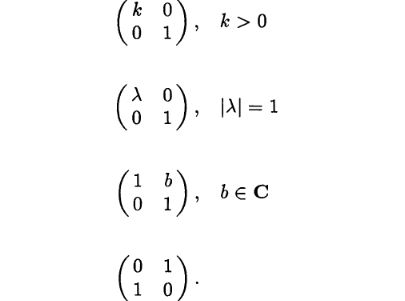
\includegraphics[width=0.5\textwidth]{graphics/p1.png}
    \end{center}
\end{tcolorbox}
\begin{marginfigure}%
    \includegraphics[width=2.3\marginparwidth]{graphics/ (24).png}
\end{marginfigure}%
Note that
\begin{enumerate}
    \item Matrix of type 1 and 2 sends $z\to re^{i\theta}z$
    \item Matrix of type 3 sends $z\to z+b$
    \item Matrix of type 4 sends $z\to1/z$ 
\end{enumerate}
Note that $\phi(z)=\frac{az+b}{cz+d}=\frac{b-ad/c}{cz+d}+\frac{a}{c}$. We can achieve this transformation by consecutive matrix multiplications as noted below:
$$z \xrightarrow[]{\text{Matrix 1,2}} cz\xrightarrow[]{\text{Matrix 3}} cz+d\xrightarrow[]{\text{Matrix 4}}\frac{1}{cz+d}\xrightarrow[]{\text{Matrix 1,2}}\frac{b-ad/c}{cz+d}\xrightarrow[]{\text{Matrix 3}}\frac{b-ad/c}{cz+d}+\frac{a}{c}$$
Note that if $c=re^{i\theta}$ then:
$$\begin{bmatrix}
    c &0\\
    0 &1
\end{bmatrix}=\begin{bmatrix}
    re^{t\theta} &0\\
    0 &1
\end{bmatrix}=\begin{bmatrix}
    r &0\\
    0 &1
\end{bmatrix}\begin{bmatrix}
    e^{t\theta} &0\\
    0 &1
\end{bmatrix}$$
We have:
$$cI=\begin{bmatrix}
    c &0\\
    0 &1
\end{bmatrix}\begin{bmatrix}
    0 &1\\
    1 &0
\end{bmatrix}\begin{bmatrix}
    c &0\\
    0 &1
\end{bmatrix}\begin{bmatrix}
    0 &1\\
    1 &0
\end{bmatrix}$$

We every matrix of $GL_2(\mathbb C)$ is a product of a matrix of form $cI$ and $\phi$ where $\phi$ is LFT. As $\phi$ and $cI$ can both be written as the product of matrices of given types, the claim is proved. 

\section{3.7-3.8}

\begin{tcolorbox}[colback=blue!15]
    \textbf{Problem}\\
    Prove that $z_1,z_2,z_3,z_4$ lie on a circle iff $(z_1,z_2;z_3,z_4)$ is real.
\end{tcolorbox}
\begin{marginfigure}%
    \includegraphics[width=2.3\marginparwidth]{graphics/ (23).png}
\end{marginfigure}%
Consider $\phi$ which transforms $z_i\to\omega_i$ for $i=1,2,3$($\omega_i$ as defined in notes). Note that the only circle passing through $\omega_1,\omega_2,\omega_3$ is the real line. Then we have from a previous problem:  
\begin{align*}
    &z_1,z_2,z_3,z_4 \text{ lie on a circle}\\
    \Leftrightarrow& \phi(z_1),\phi(z_2),\phi(z_3),\phi(z_4) \text{ lie on a circle}\\
    \Leftrightarrow& \phi(z_4)\text{ is real}
\end{align*}
Note that the map which takes $\phi(z_i)=\omega_i$ to $\omega_i$ is the identity map and $\phi(z_4)=(\phi(z_1),\phi(z_2);\phi(z_3),\phi(z_4))$ Therefore, continuing from above we have:
\begin{align*}
    \Leftrightarrow& \phi(z_4)\text{ is real}\\
    \Leftrightarrow& (\phi(z_1),\phi(z_2);\phi(z_3),\phi(z_4))\text{ is real}\\
    \Leftrightarrow& (z_1,z_2;z_3,z_4)\text{ is real}\\
\end{align*}
\section{3.9}
Those exercises are linear algebra. I hate linear algebra. \\
\newpage

\includegraphics[width=1.15\textwidth]{graphics/2-2.jpg}


\chapter{Elementary Functions}



\chapter{Power Series}


\end{document}










